\subsection{Logiciel}
	\paragraph*{}
	L'architecture logicielle des trois modules est présentée ici sous forme de pile montrant ainsi les inters dépendances entre chaque couche. La première couche est pour l'applicatif. On y trouve les différentes tâches que le module doit effectuer. Ensuite vient la couche des "middlewares", puis celle des services. Les services sont des librairies logicielles contextualisées qui utilisent les pilotes pour effectuer des tâches de plus haut niveau. Les trois dernières couches sont celles des pilotes, de l'abstraction matérielle et des périphériques matériels internes.
	\subsubsection*{Module maître}
		\noindent
		Interruption : Base de temps du HAL, base de temps du RTOS, CAN \#1 (Tx et Rx),  CAN \#2 (Tx et Rx) \\
		Interrogation : ADC externe cellules (x8), ADC interne thermistor (x2), Bouton de reprise d’erreur
		\begin{figure}[H]
			\centering
			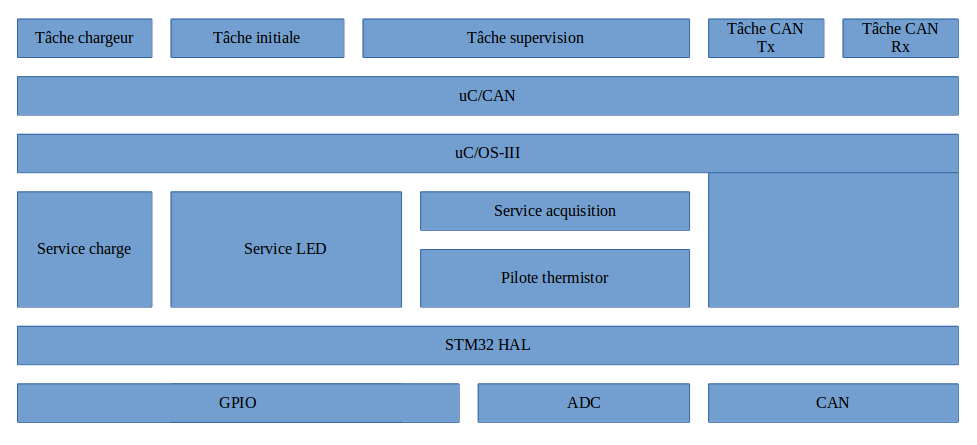
\includegraphics[scale=0.5]{Images/Logiciel_Master.png}
			\caption{Logiciel du module maître}
			\label{fig:logiciel_master}
		\end{figure}
	\subsubsection*{Module esclave}
		\noindent
		Interruption : Base de temps du HAL, base de temps du RTOS, CAN \#1 (Tx et Rx) \\
		Interrogation : ADC externe cellules (x8), ADC interne thermistor (x2)
		\begin{figure}[H]
			\centering
			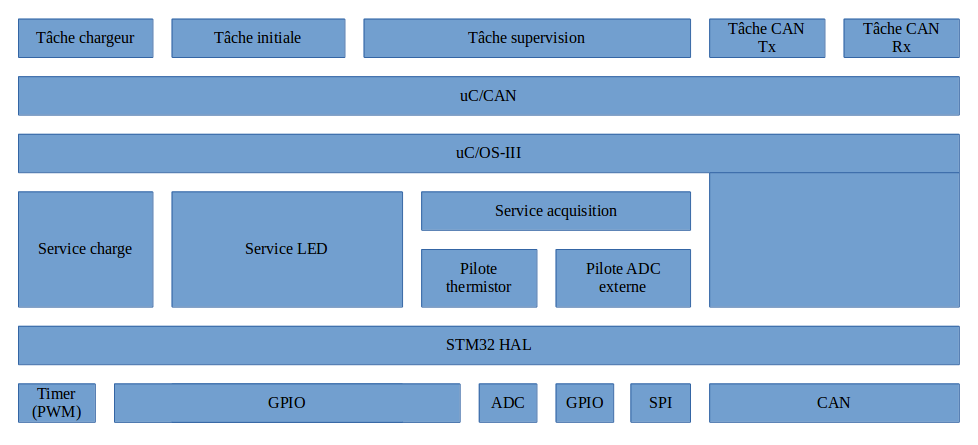
\includegraphics[scale=0.5]{Images/Logiciel_Slave.png}
			\caption{Logiciel des modules esclaves}
			\label{fig:logiciel_slave}
		\end{figure}
	\subsubsection*{Module de lecture de courant}
		\noindent
		Interruption : Base de temps du HAL, base de temps du RTOS, CAN \#1 (Tx et Rx) \\
		Interrogation : ADC externe shunt
		\begin{figure}[H]
			\centering
			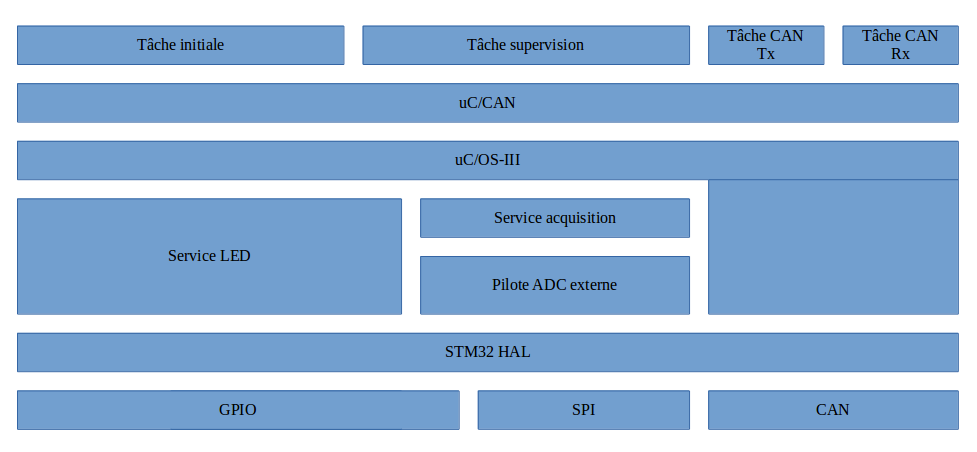
\includegraphics[scale=0.5]{Images/Logiciel_Current_Sense.png}
			\caption{Logiciel du module de lecture de courant}
			\label{fig:logiciel_current_sense}
		\end{figure}
